\documentclass{standalone}
\usepackage{tikz}
\usetikzlibrary{patterns, positioning}
\usepackage[sfdefault]{ClearSans} %% option 'sfdefault' activates Clear Sans as the default text font
\usepackage[T1]{fontenc}

\begin{document}
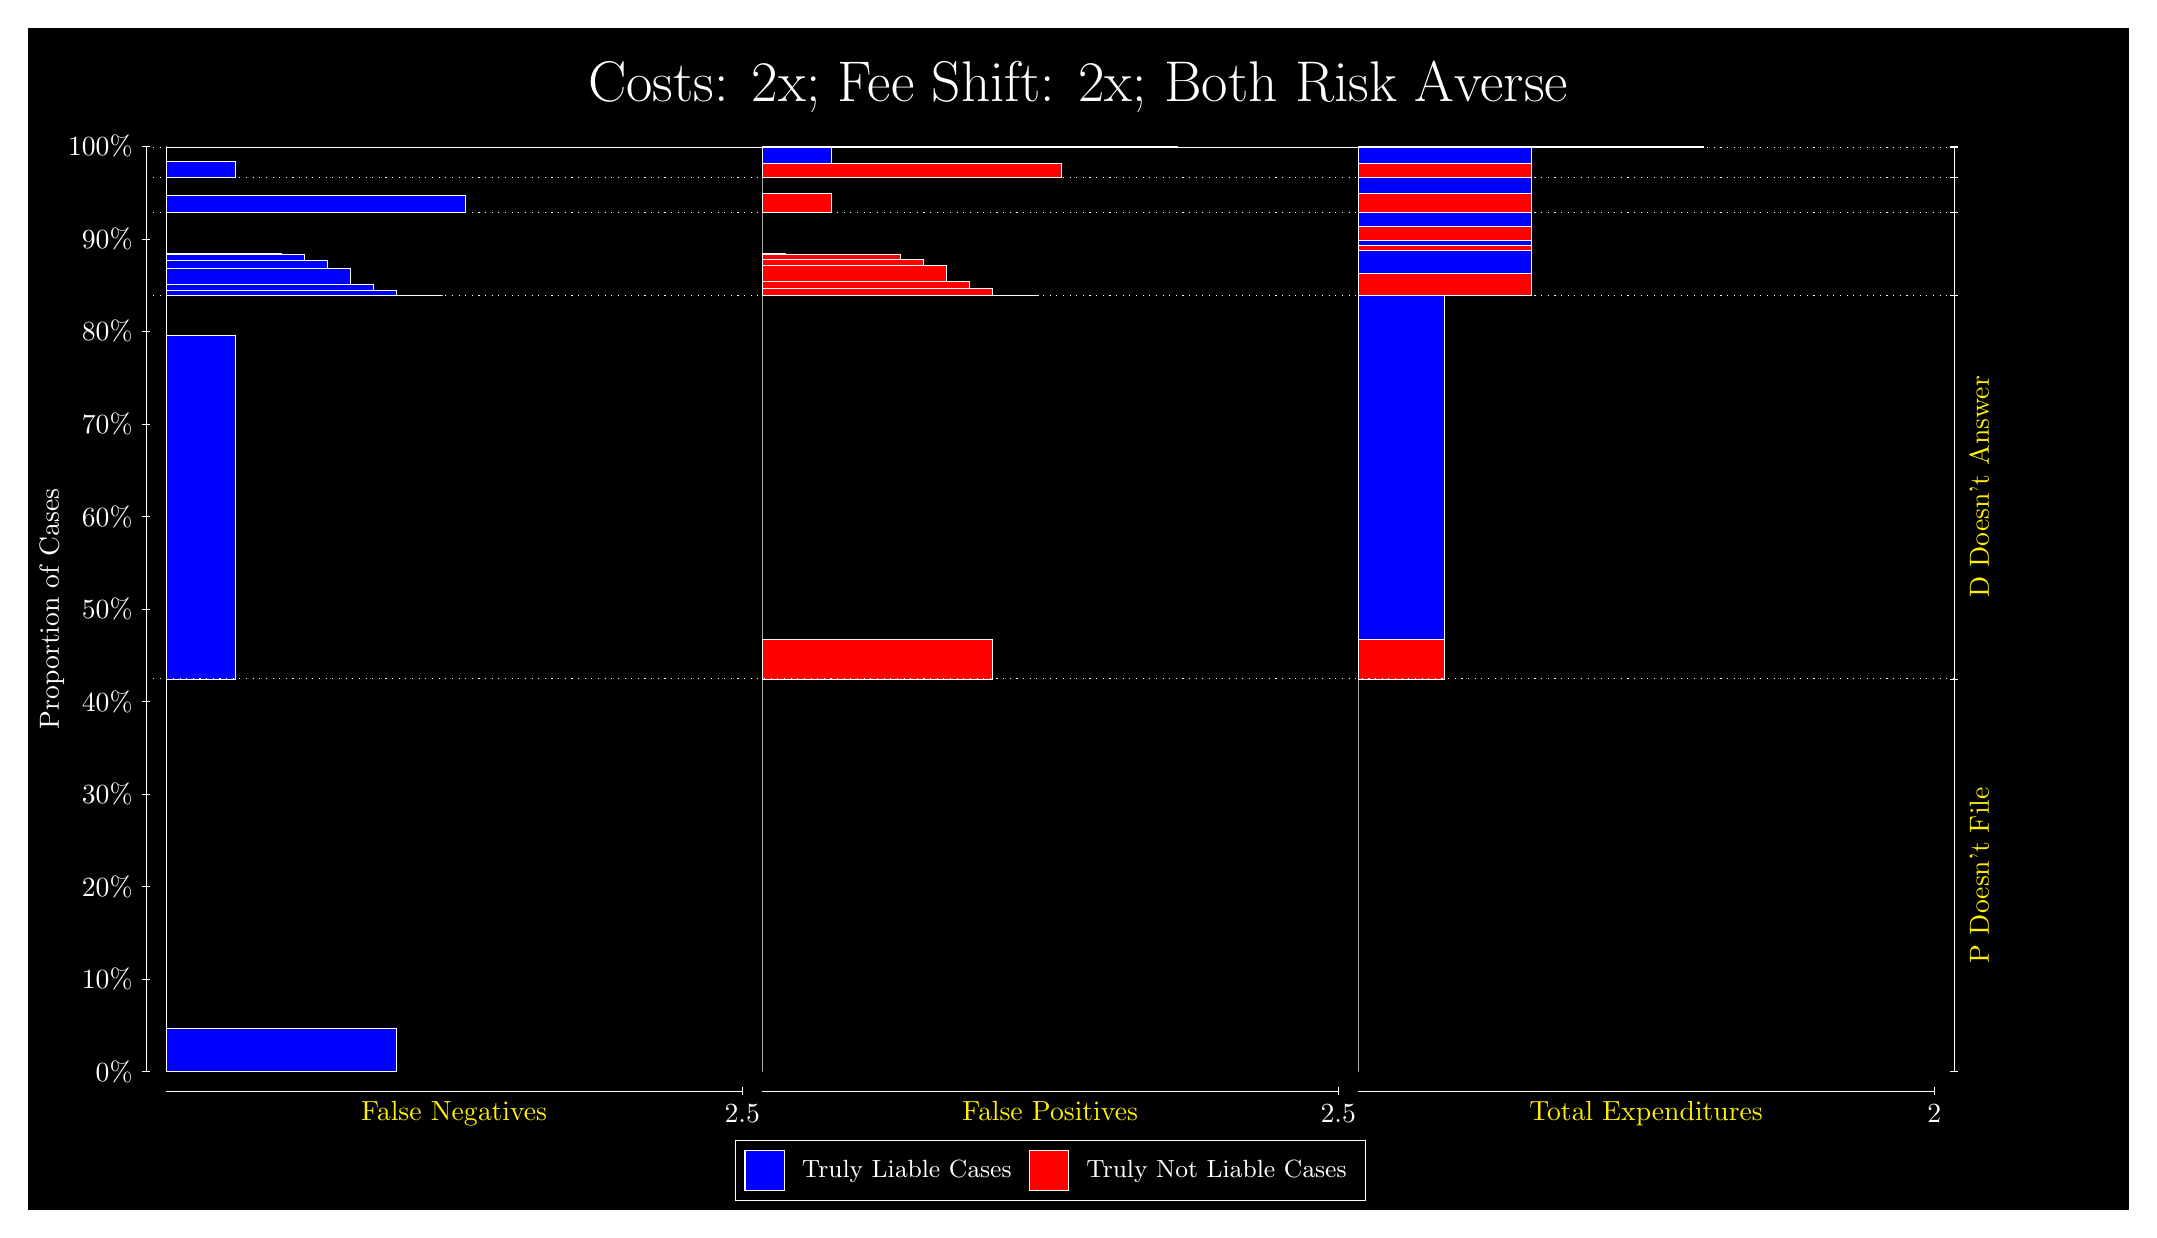
\begin{tikzpicture}
\draw[fill=black] (0,0) rectangle (26.667,15);
\draw[text=white] (0,13.5) rectangle (26.667,15) node[midway] {\huge Costs: 2x; Fee Shift: 2x; Both Risk Averse};
\draw[white, very thin] (1.5,1.75) -- (1.5,13.5);
\node[rotate=90, text=white, anchor=center] at (0.3, 7.625) {Proportion of Cases};
\draw[white, very thin] (1.45,1.75) -- (1.55,1.75);
\node[text=white, anchor=east] at (1.45, 1.75) {0\%};
\draw[white, very thin] (1.45,2.925) -- (1.55,2.925);
\node[text=white, anchor=east] at (1.45, 2.925) {10\%};
\draw[white, very thin] (1.45,4.1) -- (1.55,4.1);
\node[text=white, anchor=east] at (1.45, 4.1) {20\%};
\draw[white, very thin] (1.45,5.275) -- (1.55,5.275);
\node[text=white, anchor=east] at (1.45, 5.275) {30\%};
\draw[white, very thin] (1.45,6.45) -- (1.55,6.45);
\node[text=white, anchor=east] at (1.45, 6.45) {40\%};
\draw[white, very thin] (1.45,7.625) -- (1.55,7.625);
\node[text=white, anchor=east] at (1.45, 7.625) {50\%};
\draw[white, very thin] (1.45,8.8) -- (1.55,8.8);
\node[text=white, anchor=east] at (1.45, 8.8) {60\%};
\draw[white, very thin] (1.45,9.975) -- (1.55,9.975);
\node[text=white, anchor=east] at (1.45, 9.975) {70\%};
\draw[white, very thin] (1.45,11.15) -- (1.55,11.15);
\node[text=white, anchor=east] at (1.45, 11.15) {80\%};
\draw[white, very thin] (1.45,12.325) -- (1.55,12.325);
\node[text=white, anchor=east] at (1.45, 12.325) {90\%};
\draw[white, very thin] (1.45,13.5) -- (1.55,13.5);
\node[text=white, anchor=east] at (1.45, 13.5) {100\%};

\draw[white, very thin] (24.457,1.75) -- (24.457,13.5);
\draw[white, very thin] (24.407,1.75) -- (24.507,1.75);
\node[anchor=west] at (24.407, 1.75) {};
\draw[white, very thin] (24.407,6.7379) -- (24.507,6.7379);
\node[anchor=west] at (24.407, 6.7379) {};
\draw[white, very thin] (24.407,11.609) -- (24.507,11.609);
\node[anchor=west] at (24.407, 11.609) {};
\draw[white, very thin] (24.407,12.663) -- (24.507,12.663);
\node[anchor=west] at (24.407, 12.663) {};
\draw[white, very thin] (24.407,13.108) -- (24.507,13.108);
\node[anchor=west] at (24.407, 13.108) {};
\draw[white, very thin] (24.407,13.486) -- (24.507,13.486);
\node[anchor=west] at (24.407, 13.486) {};
\draw[white, very thin] (24.407,13.487) -- (24.507,13.487);
\node[anchor=west] at (24.407, 13.487) {};
\draw[white, very thin] (24.407,13.5) -- (24.507,13.5);
\node[anchor=west] at (24.407, 13.5) {};

\draw[white, very thin, fill=blue] (1.75,1.75) rectangle (4.6775,2.2998);
\draw[white, very thin, fill=red] (1.75,2.2998) rectangle (1.75,6.7379);
\draw[white, very thin, fill=blue] (1.75,6.7379) rectangle (2.6283,11.104);
\draw[white, very thin, fill=red] (1.75,11.104) rectangle (1.75,11.609);
\draw[white, very thin, fill=blue] (1.75,11.609) rectangle (5.2631,11.609);
\draw[white, very thin, fill=blue] (1.75,11.609) rectangle (4.9703,11.61);
\draw[white, very thin, fill=blue] (1.75,11.61) rectangle (4.6775,11.672);
\draw[white, very thin, fill=blue] (1.75,11.672) rectangle (4.3848,11.673);
\draw[white, very thin, fill=blue] (1.75,11.673) rectangle (4.3848,11.753);
\draw[white, very thin, fill=blue] (1.75,11.753) rectangle (4.092,11.95);
\draw[white, very thin, fill=blue] (1.75,11.95) rectangle (3.7993,12.047);
\draw[white, very thin, fill=blue] (1.75,12.047) rectangle (3.5065,12.135);
\draw[white, very thin, fill=blue] (1.75,12.135) rectangle (3.2138,12.139);
\draw[white, very thin, fill=blue] (1.75,12.139) rectangle (2.921,12.142);
\draw[white, very thin, fill=red] (1.75,12.142) rectangle (1.75,12.663);
\draw[white, very thin, fill=blue] (1.75,12.663) rectangle (5.5558,12.872);
\draw[white, very thin, fill=red] (1.75,12.872) rectangle (1.75,13.108);
\draw[white, very thin, fill=blue] (1.75,13.108) rectangle (2.6283,13.312);
\draw[white, very thin, fill=red] (1.75,13.312) rectangle (1.75,13.486);
\draw[white, very thin, fill=blue] (1.75,13.486) rectangle (9.9471,13.487);
\draw[white, very thin, fill=red] (1.75,13.487) rectangle (1.75,13.487);
\draw[white, very thin, fill=red] (1.75,13.487) rectangle (1.75,13.49);
\draw[white, very thin, fill=blue] (1.75,13.49) rectangle (1.75,13.5);
\draw[white, very thin, fill=red] (9.3189,1.75) rectangle (9.3189,6.1881);
\draw[white, very thin, fill=blue] (9.3189,6.1881) rectangle (9.3189,6.7379);
\draw[white, very thin, fill=red] (9.3189,6.7379) rectangle (12.246,7.2423);
\draw[white, very thin, fill=blue] (9.3189,7.2423) rectangle (9.3189,11.609);
\draw[white, very thin, fill=red] (9.3189,11.609) rectangle (12.832,11.61);
\draw[white, very thin, fill=red] (9.3189,11.61) rectangle (12.539,11.612);
\draw[white, very thin, fill=red] (9.3189,11.612) rectangle (12.246,11.696);
\draw[white, very thin, fill=red] (9.3189,11.696) rectangle (11.954,11.792);
\draw[white, very thin, fill=red] (9.3189,11.792) rectangle (11.661,11.987);
\draw[white, very thin, fill=red] (9.3189,11.987) rectangle (11.368,12.066);
\draw[white, very thin, fill=red] (9.3189,12.066) rectangle (11.075,12.129);
\draw[white, very thin, fill=red] (9.3189,12.129) rectangle (10.783,12.129);
\draw[white, very thin, fill=red] (9.3189,12.129) rectangle (10.49,12.129);
\draw[white, very thin, fill=blue] (9.3189,12.129) rectangle (9.9044,12.133);
\draw[white, very thin, fill=blue] (9.3189,12.133) rectangle (9.6116,12.137);
\draw[white, very thin, fill=blue] (9.3189,12.137) rectangle (9.3189,12.663);
\draw[white, very thin, fill=red] (9.3189,12.663) rectangle (10.197,12.898);
\draw[white, very thin, fill=blue] (9.3189,12.898) rectangle (9.3189,13.108);
\draw[white, very thin, fill=red] (9.3189,13.108) rectangle (13.125,13.281);
\draw[white, very thin, fill=blue] (9.3189,13.281) rectangle (10.197,13.486);
\draw[white, very thin, fill=red] (9.3189,13.486) rectangle (9.3189,13.487);
\draw[white, very thin, fill=blue] (9.3189,13.487) rectangle (9.3189,13.487);
\draw[white, very thin, fill=red] (9.3189,13.487) rectangle (17.516,13.49);
\draw[white, very thin, fill=blue] (9.3189,13.49) rectangle (14.588,13.5);
\draw[white, very thin, fill=red] (16.888,1.75) rectangle (16.888,6.1881);
\draw[white, very thin, fill=blue] (16.888,6.1881) rectangle (16.888,6.7379);
\draw[white, very thin, fill=red] (16.888,6.7379) rectangle (17.986,7.2423);
\draw[white, very thin, fill=blue] (16.888,7.2423) rectangle (17.986,11.609);
\draw[white, very thin, fill=red] (16.888,11.609) rectangle (19.083,11.89);
\draw[white, very thin, fill=blue] (16.888,11.89) rectangle (19.083,12.179);
\draw[white, very thin, fill=red] (16.888,12.179) rectangle (19.083,12.243);
\draw[white, very thin, fill=blue] (16.888,12.243) rectangle (19.083,12.307);
\draw[white, very thin, fill=red] (16.888,12.307) rectangle (19.083,12.482);
\draw[white, very thin, fill=blue] (16.888,12.482) rectangle (19.083,12.663);
\draw[white, very thin, fill=red] (16.888,12.663) rectangle (19.083,12.898);
\draw[white, very thin, fill=blue] (16.888,12.898) rectangle (19.083,13.108);
\draw[white, very thin, fill=red] (16.888,13.108) rectangle (19.083,13.281);
\draw[white, very thin, fill=blue] (16.888,13.281) rectangle (19.083,13.486);
\draw[white, very thin, fill=red] (16.888,13.486) rectangle (21.279,13.487);
\draw[white, very thin, fill=blue] (16.888,13.487) rectangle (21.279,13.487);
\draw[white, very thin, fill=red] (16.888,13.487) rectangle (21.279,13.49);
\draw[white, very thin, fill=blue] (16.888,13.49) rectangle (21.279,13.5);
\draw[white, dotted] (1.5,6.7379) -- (24.457,6.7379);
\draw[white, dotted] (1.5,11.609) -- (24.457,11.609);
\draw[white, dotted] (1.5,12.663) -- (24.457,12.663);
\draw[white, dotted] (1.5,13.108) -- (24.457,13.108);
\draw[white, dotted] (1.5,13.486) -- (24.457,13.486);
\draw[white, dotted] (1.5,13.487) -- (24.457,13.487);
\draw[white, very thin] (1.75,1.5) -- (9.0689,1.5);
\node[text=yellow, anchor=north] at (5.4094, 1.5) {False Negatives};
\draw[white, very thin] (9.0689,1.45) -- (9.0689,1.55);
\node[text=white, anchor=north] at (9.0689, 1.45) {2.5};

\draw[white, very thin] (9.3189,1.5) -- (16.638,1.5);
\node[text=yellow, anchor=north] at (12.978, 1.5) {False Positives};
\draw[white, very thin] (16.638,1.45) -- (16.638,1.55);
\node[text=white, anchor=north] at (16.638, 1.45) {2.5};

\draw[white, very thin] (16.888,1.5) -- (24.207,1.5);
\node[text=yellow, anchor=north] at (20.547, 1.5) {Total Expenditures};
\draw[white, very thin] (24.207,1.45) -- (24.207,1.55);
\node[text=white, anchor=north] at (24.207, 1.45) {2};

\node[text=yellow, centered, rotate=90] at (24.777, 4.2439) {P Doesn't File};
\node[text=yellow, centered, rotate=90] at (24.777, 9.1734) {D Doesn't Answer};






\draw (12.978300999999998,1.5) node[draw=none] (baseCoordinate) {};
\begin{scope}[align=center]
        \matrix[scale=0.5, draw=white, below=0.5cm of baseCoordinate, nodes={draw}, column sep=0.1cm]{
            \node[rectangle, draw, minimum width=0.5cm, minimum height=0.5cm, fill=blue] {}; &
            \node[draw=none, font=\small, text=white] (B) {Truly Liable Cases}; &
            \node[rectangle, draw, minimum width=0.5cm, minimum height=0.5cm, fill=red] {}; &
            \node[draw=none, font=\small, text=white] (B) {Truly Not Liable Cases}; \\
            };
\end{scope}

\end{tikzpicture}
\end{document}